\documentclass[10pt, landscape]{article}
\usepackage[scaled=0.92]{helvet}
\usepackage{calc}
\usepackage{multicol}
\usepackage{ifthen}
\usepackage[a4paper,margin=3mm,landscape]{geometry}
\usepackage{amsmath,amsthm,amsfonts,amssymb}
\usepackage{color,graphicx,overpic}
\usepackage{hyperref}
\usepackage{newtxtext} 
\usepackage{enumitem}
\usepackage{amssymb}
\usepackage[table]{xcolor}
\usepackage{vwcol}
\usepackage{tikz}
\usetikzlibrary{arrows.meta}
\usetikzlibrary{calc}
\usepackage{mathtools}
\usepackage{nicematrix}
% for relations
\usepackage{cancel}
\usepackage{ mathrsfs }
\graphicspath{ {./images/} }
\setlist{nosep}

\pdfinfo{
  /Title (CS1231.pdf)
  /Creator (TeX)
  /Producer (pdfTeX 1.40.0)
  /Author (Seamus)
  /Subject (Example)
  /Keywords (pdflatex, latex,pdftex,tex)}

% Turn off header and footer
\pagestyle{empty}

\newenvironment{tightcenter}{%
  \setlength\topsep{0pt}
  \setlength\parskip{0pt}
  \begin{center}
}{%
  \end{center}
}

% redefine section commands to use less space
\makeatletter
\renewcommand{\section}{\@startsection{section}{1}{0mm}%
                                {-1ex plus -.5ex minus -.2ex}%
                                {0.5ex plus .2ex}%x
                                {\normalfont\large\bfseries}}
\renewcommand{\subsection}{\@startsection{subsection}{2}{0mm}%
                                {-1explus -.5ex minus -.2ex}%
                                {0.5ex plus .2ex}%
                                {\normalfont\normalsize\bfseries}}
\renewcommand{\subsubsection}{\@startsection{subsubsection}{3}{0mm}%
                                {-1ex plus -.5ex minus -.2ex}%
                                {1ex plus .2ex}%
                                {\normalfont\small\bfseries}}%
\renewcommand{\familydefault}{\sfdefault}
\renewcommand\rmdefault{\sfdefault}
% makes nested numbering (e.g. 1.1.1, 1.1.2, etc)
\renewcommand{\labelenumii}{\theenumii}
\renewcommand{\theenumii}{\theenumi.\arabic{enumii}.}
\renewcommand\labelitemii{•}
%  for logical not operator
\renewcommand{\lnot}{\mathord{\sim}}
\renewcommand{\bf}[1]{\textbf{#1}}
\newcommand{\abs}[1]{\vert #1 \vert}
\newcommand{\Mod}[1]{\ \mathrm{mod}\ #1}

\makeatother
\definecolor{myblue}{cmyk}{1,.72,0,.38}
\everymath\expandafter{\the\everymath \color{myblue}}
% Define BibTeX command
\def\BibTeX{{\rm B\kern-.05em{\sc i\kern-.025em b}\kern-.08em
    T\kern-.1667em\lower.7ex\hbox{E}\kern-.125emX}}
\let\iff\leftrightarrow
\let\Iff\Leftrightarrow
\let\then\rightarrow
\let\Then\Rightarrow

% Don't print section numbers
\setcounter{secnumdepth}{0}

\setlength{\parindent}{0pt}
\setlength{\parskip}{0pt plus 0.5ex}
%% this changes all items (enumerate and itemize)
\setlength{\leftmargini}{0.5cm}
\setlength{\leftmarginii}{0.5cm}
\setlist[itemize,1]{leftmargin=2mm,labelindent=1mm,labelsep=1mm}
\setlist[itemize,2]{leftmargin=4mm,labelindent=1mm,labelsep=1mm}

%My Environments
\newtheorem{example}[section]{Example}
% -----------------------------------------------------------------------

\begin{document}
\raggedright
\footnotesize
\begin{multicols}{4}


% multicol parameters
% These lengths are set only within the two main columns
\setlength{\columnseprule}{0.25pt}
\setlength{\premulticols}{1pt}
\setlength{\postmulticols}{1pt}
\setlength{\multicolsep}{1pt}
\setlength{\columnsep}{2pt}

\begin{center}
    \fbox{%
        \parbox{0.8\linewidth}{\centering \textcolor{black}{
            {\Large\textbf{CS1231}}
            \\ \normalsize{AY22/23 sem 2}}
            \\ {\footnotesize \textcolor{myblue}{github.com/NeoHW}} 
        }%
    }
\end{center}

\section{01. Propositional Logic}
\subsection{sets of numbers}
    $\mathbb{N}$ : natural numbers ($\mathbb{Z}_{\geq 0}$)
\\* $\mathbb{Z}$ : integers
\\* $\mathbb{Q}$ : rational numbers
\\* $\mathbb{R}$ : real numbers
\\* $\mathbb{C}$ : complex numbers
\\* $\mathbb{N} \subseteq \mathbb{Z} \subseteq \mathbb{Q} \subseteq \mathbb{R} \subseteq \mathbb{C}$

\subsection{basic properties of integers}
\begin{center}
    closure (under addition and multiplication)
    \\* $x+y \in \mathbb{Z} \land xy \in \mathbb{Z}$

    commutativity
    \\* $a + b = b + a \land ab = ba$

    associativity
    \\* $a + b + c = a + (b + c) = (a + b) + c$
    \\* $abc = a(bc) = (ab)c$

    distributivity
    \\* $a(b + c) = ab + ac$

    trichotomy
    \\* $(a < b) \lor (a > b) \lor (a = b)$

    transitive law
    \\* $(a < b) \land (b < c) \implies (a < c)$
\end{center}
 
\subsection{definitions}
\begin{center}
    even/odd
    \\* $n \text{ is even} \iff \exists k \in \mathbb{Z} \mid n = 2k$
    \\* $n \text{ is odd} \iff \exists k \in \mathbb{Z} \mid n = 2k + 1$

    prime/composite
    \\* $n \text{ is prime} \iff n>1 \text{ and } \forall r, s \in \mathbb{Z}^+, n=rs \then (r=n)\lor(r=s)$
    \\* $n \text{ is composite} \iff n>1 \text{ and } \exists r, s \in \mathbb{Z}^+ s.t. n = rs \text{ and } 1<r<n \text{ and } 1<s<n$

    divisibility ($d$ divides $n$)
    \\* $d \mid n \iff \exists k \in \mathbb{Z} \mid n = kd$

    rationality
    \\* $r \text{ is rational} \iff \exists a, b \in \mathbb{Z} \mid r = \frac{a}{b} \text{ and } b \neq 0$

    floor/ceiling
    \\* $\lfloor x \rfloor$ : largest integer $y$ such that $y \leq x$
    \\* $\lceil x \rceil$ : smallest integer $y$ such that $y \geq x$
\subsubsection{rules of inference}
    \begin{multicols}{2}
        generalisation
        \\* $p,\ \therefore p \lor q$
        
        specialisation
        \\* $p \land q,\ \therefore p$

        elimination
        \\* $p \lor q;\ \ \lnot q,\ \therefore p$

        transitivity
        \\* $p \then q;\ q \then r;\ \ \therefore p \then r$
    \end{multicols}
\end{center}

\section{03. PROOFS}
\subsection{Proof by Exhaustion/Cases}
\begin{enumerate}
    \item list out possible cases
    \begin{enumerate}
        \item Case 1: $n$ is odd OR If $n = 9$, ...
        \item Case 2: $n$ is even OR If $n = 16$, ...
    \end{enumerate}
    \item therefore ...
\end{enumerate}

\subsection{Proof by Contradiction}
\begin{enumerate}
    \item Suppose that \dots
    \begin{enumerate}
        \item <proof>
        \item \dots but this contradicts \dots
    \end{enumerate}
    \item Therefore the assumption that \dots is false. \\* Hence \dots.
\end{enumerate}

\subsection{Proof by Contraposition}
\begin{enumerate}
    \item Contrapositive statement: $\lnot q \then \lnot p$
    \item let $\lnot q$
    \begin{enumerate}
        \item <proof>
        \item hence $\lnot p$
    \end{enumerate}
    \item $\therefore p \then q$
\end{enumerate}

\subsection{Proof by Construction}
\begin{enumerate}
    \item Let $x = 3, y=4, z=5$.
    \item Then $x, y, z \in \mathbb{Z}_{\geq 1}$ and $x^2 + y^2 = 3^2 + 4^2 = 9 + 16 = 25 = 5^2$.
    \item Thus $\exists x, y, z \in \mathbb{Z}_{\geq 1}$ such that $x^2 + y^2 = z^2$.
\end{enumerate}

\subsection{Proof by Induction}
\begin{enumerate}
    \item For each $n \in \mathbb{Z}_{\geq 1}$, let $P(n)$ be the proposition "$\dots$"
    \item (base step) $P(1)$ is true because <manual method>
    \item (induction step) 
    \begin{enumerate}
        \item let $k \in \mathbb{Z}_{\geq 1}$ s.t. $P(k)$ is true
        \item Then \dots
        \item proof that $P(k + 1)$ is true - e.g. $P(k+1) = P(k) + term_{k+1}$
        \item So $P(k + 1)$ is true.
    \end{enumerate}
    \item Hence $\forall n \in \mathbb{Z}_{\geq 1} P(n)$ is true by MI.
\end{enumerate}

\subsection{INDUCTION}
\subsection{mathematical induction}
to prove that $\forall n \in \mathbb{Z}_{\geq m} (P(n))$ is true, 
\begin{itemize}
    \item base step: show that $P(m)$ is true
    \item induction step: show that $\forall k \in \mathbb{Z}_{\geq m} (P(k) \Rightarrow P(k + 1))$ is true.
    \begin{itemize}
        \item induction hypothesis: assumption that $P(k)$ is true 
    \end{itemize}
\end{itemize}

\subsection{strong MI}
to prove that $\forall n \in \mathbb{Z}_{\geq 0} (P(n))$ is true, 
\begin{itemize}
    \item base step: show that $P(0), P(1)$ are true
    \item induction step: show that $\forall k \in \mathbb{Z}_{\geq 0} (P(0) \dots \land P(k+1) \Rightarrow P(k + 2))$ is true.
\end{itemize}
justification:
\begin{itemize}
    \item $P(0) \land P(1)$ by base case
    \item $P(0) \land P(1) \then P(2)$ by induction with $k=0$
    \item $P(0) \land P(1) \land P(2) \then P(3)$ by induction with $k=1$
    \item $\ \ \ \dotsm $ 
    \item we deduce that $P(0), P(1), \dots $ are all true by a series of \bf{modus ponens}
\end{itemize}

\subsection{Proofs for Sets}
\bf{Equality of Sets (A=B)}
\begin{enumerate}
    \item $(\Rightarrow)$
        \begin{enumerate}
            \item Take any $z \in A$.
            \item $\dots$
            \item $\therefore z \in B$.
        \end{enumerate}
    \item $(\Leftarrow)$
    \begin{enumerate}
        \item Take any $z \in B$.
        \item $\dots$
        \item $\therefore z \in A$.
    \end{enumerate}
\end{enumerate}

\bf{Element Method}
\begin{enumerate}
    \item $A \cap (B \backslash C) = \{ x : x \in A \land x \in (B \backslash C) \}$ (by def. of $\cap$)
    \item $= \{ x : x \in A \land (x \in B \land x \notin C)\}$ (by def. of $\backslash$)
    \item $\dots$
    \item $= (A \cap B) \backslash C$ (by def. of $\backslash$)
\end{enumerate}

\subsection{Other Proofs}
\bf{iff ($A \iff B$)}
\begin{enumerate}
    \item ($\Rightarrow$) Suppose $A$.
    \begin{enumerate}
        \item $\dots$ <proof> $\dots$
        \item Hence $A \then B$
    \end{enumerate}
    \item ($\Leftarrow$) Suppose $B$.
    \begin{enumerate}
        \item $\dots$ <proof> $\dots$
        \item Hence $B \then A$
    \end{enumerate}
\end{enumerate}

\section{02. PREDICATE LOGIC}
\subsection{operations}
\begin{itemize}
    \item[1] $\sim$ : negation (not)
    \item[2] $\land$ : conjunction (and)
    \item[2] $\lor$ : disjunction (or) - coequal to $\land$
    \item[3] $\rightarrow$ : if-then
\end{itemize}

\subsubsection{logical equivalence} 
\begin{itemize}
    \item identical truth values in truth table
    \item definitions
    \item to show non-equivalence: 
    \begin{itemize}
        \item truth table method (only needs 1 row)
        \item counter-example method
    \end{itemize}
\end{itemize}

\subsection{conditional statements}
    \begin{equation*}
        \begin{split}
            \text{hypothesis} &\then \text{conclusion} \\
            antecedent &\then consequent
        \end{split}
    \end{equation*}

\begin{itemize}
    \item \textbf{vacuously true} : hypothesis is false
    \item \textbf{implication law} : $p \then q \equiv \lnot p \lor q$
    \item common statements for $p \then q$ :
    \begin{itemize}
        \item if p then q
        \item q if p
        \item p only if q
        \item p iff q
        \item p is sufficient for q
        \item q is necessary for p
    \end{itemize}
\end{itemize}

\begin{multicols}{2}
    \begin{itemize}
        \item \bf{contrapositive} : $\lnot q \then \lnot p$ 
        \item \bf{inverse} : $\lnot p \then \lnot q$ 
        \item \bf{converse} : $q \then p$ 
    \end{itemize} 
    \begin{center}
        statement $\equiv$ contrapositive 
        \\ converse $\equiv$ inverse 
    \end{center}
\end{multicols}
\begin{itemize}
    \item r is a \bf{necessary} condition for s: $\lnot r \then \lnot s$ and $s \then r$
    \item r is a \bf{sufficient} condition for s: $r \then s$
    \item \bf{necessary} \& \bf{sufficient} : $\iff$
\end{itemize}

\subsection{valid arguments}
\begin{itemize}
    \item determining validity: construct truth table
    \begin{itemize}
        \item valid $\iff$ conclusion is true when premises are true
    \end{itemize}
    \item \bf{syllogism} : (argument form) 2 premises, 1 conclusion
    \item \bf{modus ponens} : $p \then q;\ p;\ \therefore q$
    \item \bf{modus tollens} : $p \then q;\ \lnot q;\ \therefore \lnot p$
    \item \bf{sound argument} : is valid \& all premises are true
\end{itemize}

\subsection{fallacies}
\begin{center}
    \begin{multicols}{2}
        converse error \\*
        $p \then q$ \\ $q$ \\ $\therefore p$

        inverse error \\*
        $p \then q$ \\ $\lnot p$ \\ $\therefore \lnot q$
    \end{multicols}
\end{center}

\section{QUANTIFIED STATEMENTS}
\begin{itemize}
    \item \bf{truth set} of $P(x) = \{x \in D \mid P(x)\}$
    \item $P(x) \Rightarrow Q(x)$ : $\forall x (P(x) \then Q(x))$
\item $P(x) \Leftrightarrow Q(x)$ : $\forall x (P(x) \iff Q(x))$
\end{itemize}
\bf{relation between $\forall, \exists, \land, \lor$}
\begin{itemize}
    \item $\forall x \in D, Q(x) \equiv Q(x_1) \land Q(x_2) \land \dots \land Q(x_n)$
    \item $\exists x \in D \mid Q(x) \equiv Q(x_1) \lor Q(x_2) \lor \dots \lor Q(x_n)$
\end{itemize}
\bf{relation between $\lnot, \forall, \exists$}
\begin{itemize}
    \item $ \lnot \forall \: P(x) \iff \exists x \: \lnot P(x)$
    \item $ \lnot \exists \: P(x) \iff \forall x \: \lnot P(x)$
\end{itemize}



\section{04. SETS}
\subsection{notation}
\begin{itemize}
    \item set roster notation [1]: $\{x_1, x_2, \dots, x_n\}$
    \item set roster notation [2]: $\{x_1, x_2, x_3, \dots\}$
    \item set-builder notation: $\{x \in \mathbb{U} : P(x)\}$
    \item replacement notation: $\{t(x) : x \in A \}$
\end{itemize}

\subsection{definitions}
\begin{itemize}
    \item \bf{equal sets} : $A = B \iff \forall x (x \in A \iff x \in B)$ 
    \begin{itemize}
        \item $A = B \iff (A \subseteq B) \land (A \supseteq B)$
        \item order and repetition does not matter
    \end{itemize}
    \item \bf{subset} : $A \subseteq B \iff \forall x(x \in A \then x \in B)$
    \item \bf{proper subset} : $A \subsetneq B \iff (A \subseteq B) \land (A \neq B)$
    \item \bf{power set} of A : $\mathcal{P}(A) = \{X \mid X \subseteq A\}$
    \begin{itemize}
        \item $\vert \mathcal{P}(A) \vert = 2^{\vert A \vert}$, given that A is a finite set
        \item $\mathcal{P}(\emptyset) = \{\emptyset\}$ ; $\mathcal{P}(\mathcal{P}(\emptyset)) = \{\emptyset , \{\emptyset\}\}$
        \item $\mathcal{P}(\{1,2\}) = \{\emptyset, \{1\}, \{2\}, \{1,2\} \}$
    \end{itemize}
    \item \bf{cardinality} of a set, $\mid A \mid$ : number of distinct elements
    \item \bf{singleton} : sets of size 1
    \item \bf{disjoint} : $A \cap B = \emptyset$
\end{itemize}

\subsubsection{methods of proof for sets}
\begin{itemize}
    \item direct proof
    \item element method
    \item truth table
\end{itemize}

\subsubsection{boolean operations}
\begin{itemize}
    \item \bf{union:} $A \cup B = \{x : x \in A \lor x \in B\}$
    \item \bf{intersection: } $A \cap B = \{x : x \in A \land x \in B\}$
    \item \bf{complement} (of B in A): $A \backslash B = \{x : x \in A \land x \notin B\}$
    \item \bf{complement} (of B): $\bar{B}$ or $B^c = U \backslash B$
    \begin{itemize}
        \item set difference law: $A \backslash B = A \cap \bar{B}$
    \end{itemize}
\end{itemize}

\section{05. RELATIONS}
\subsection{ordered pairs}
\begin{itemize}
    \item \bf{ordered pair} : $(x, y)$
    \begin{itemize}
        \item $(x, y) = (x', y') \iff x = x' \text{ and } y = y'$
    \end{itemize}
    \item \bf{Cartesian product} : $A \times B = \{(x, y) : x \in A \text{ and } y \in B\} $
    \begin{itemize}
        \item $\vert A \times B \vert = \vert A \vert \times \vert B \vert$
        \item $\{a,b\} \times \{1,2,3\} = \{(a,1), (a,2), (a,3), (b,1), (b,2), (b,3)\}$
    \end{itemize}
    \item \bf{ordered tuples} : expression of the form $(x_1, x_2, \dots, x_n)$
    \item defined recursively : $(x_1, x_2, \dots, x_{n+1}) = ((x_1, x_2, \dots, x_n), x_{n+1})$
    \item $(1,2,5) \neq (2,1,5)$ although $\{1,2,5\} = \{2,1,5\}$
\end{itemize}

\subsection{relations}
\begin{center}
    Let $R$ be a relation from $A$ to $B$ and $(x, y) \in A \times B$. Then:
    \\* $x R y$ for $(x, y) \in R$ and $x \cancel{R} y$ for $(x, y) \notin R$
\end{center}
\begin{itemize}
    \item a relation from $A$ to $B$ is a subset of $A \times B$.
    \item a \textbf{(binary) relation} on set A is a relation from A to A.
    \begin{itemize}
        \item subset of $A^2$
    \end{itemize}
    \item \textbf{inverse relation}: $x R^{-1} y \Iff yRx$
\end{itemize}

\subsection{operations on relations}
\begin{itemize}
    \item $S \circ R = $ undergo R relation then S relation
    \item $(S \circ R)^{-1} = R^{-1} \circ S^{-1}$
\end{itemize}

\section{06. EQUIVALENCE RELATIONS AND PARTIAL ORDERS} %
\subsection{reflexivity, symmetry, transitivity}
Let $A$ be a set and $R$ be a relation on $A$.
\begin{center}
    reflexive
    \\* $\forall x \in A \ (x R x)$
    \\ symmetric
    \\* $\forall x, y \in A \ (xRy \Then y R x)$
    \\ transitive
    \\* $\forall x, y, z \in A \ (xRy \land yRz \Then xRz)$
\end{center}

\begin{itemize}
    \item \textbf{equivalence relation}: a relation that is reflexive, symmetric and transitive
    \item \textbf{equivalence class}: the set of all things equivalent to x
\end{itemize}

\subsection{equivalence classes}
Let $A$ be a set and $R$ be an equivalence relation on $A$.
\begin{itemize}
    \item $[x]_{\lnot}$ : \textbf{equivalence class} of $x$ with respect to $R$
    \begin{itemize}
        \item the set of all elements of A that x is related to
    \end{itemize}
        \centerline{$\forall x \in A, [x]_{\lnot} = \{y \in A : x R y\}$}

    \item $A / \lnot$ : The set of all equivalent classes

        \centerline{$A / R = \{[x]_{\lnot} : x \in A\}$}

\end{itemize}
$xRy \Then [x] = [y] \Then [x] \cap [y] \neq \emptyset$

\subsection{partitions}
\begin{itemize}
    \item a \textbf{partition} of a set $A$ is a set $\mathscr{C}$ of \textit{non-empty subsets} of $A$ such that
        \\ 0. $\forall S \in \mathscr{C}, \ (\emptyset \neq S \subseteq A)$
        \begin{itemize}
            \item $\mathscr{C}$ is a set of nonempty subsets of $A$
        \end{itemize}
        1. $\forall x \in A, \ \exists S \in \mathscr{C} (x \in S)$
        \begin{itemize}
            \item every element of $A$ is in some element of $\mathscr{C}$
        \end{itemize}
        2. $\forall x \in A, \ \forall S_1, S_2 \in \mathscr{C} (x \in S_1 \land x \in S_2 \Then S_1 = S_2)$
        \begin{itemize}
            \item if two items of $\mathscr{C}$ have a nonempty intersection, then they are equal
        \end{itemize}
    \item \textbf{components} : elements of a partition
    \item every partition comes from an equivalence relation
\end{itemize}

\subsection{partial orders}
Let $A$ be a set and $R$ be a relation on $A$.
\begin{itemize}
    \item $R$ is \bf{antisymmetric} if $\forall x, y \in A \ (x R y \land y R x \then x = y)$
    \begin{itemize}
        \item includes vacuously true cases (e.g. $xRy \Iff x < y$)
    \end{itemize}
    \item $R$ is a \bf{(non-strict) partial order} if $R$ is reflexive, antisymmetric and transitive.
    \item $x$ and $y$ are \bf{comparable} if $\forall x, y \in A \ (xRy \lor yRx)$
    \item $R$ is a \bf{(non-strict) total order} if $R$ is a partial order and every pair of elements are comparable
    \item a smallest element of $A$ is an element $m \in A$ such that $m R x$ for all $x \in A$
\end{itemize}

\subsection{well-ordering principle}
\begin{itemize}
    \item every nonempty subset of $\mathbb{Z}_{\geq 0}$ has a smallest element.
    \item application: recursion has a base case
\end{itemize}

\section{07. FUNCTIONS}
\subsection{definitions}
\begin{itemize}
    \item \bf{function/map} from A to B : each element of A exactly $f$-related to one element of B.
        \begin{itemize}
            \item \bf{Important} : $(x,y) \in f \iff y = f(x)$
            \item (F1): every element in A $f$-related to at least one of B
            $ \forall x \in A \: \exists y \in B \:\: (x,y) \in f$
            \item (F2): every element in A $f$-related to at most one of B
            $ \forall x \in A \: \exists y_1,y_2 \in B \:\: ((x,y_1) \in f \land (x,y_1) \in f \then y_1 = y_2)$
            \item $f:A \to B$ : "$f$ is a function from $A$ to $B$"
            \item $f:x \to y$ : "$f$ maps $x$ to $y$"
            \item \bf{domain} of f = $A$
            \item \bf{codomain} of f = $B$
            \item \bf{range/image} of f = $\{f(x) : x \in A\} $ 
                \\$= \{y \in B \mid y= f(x) \text{ for some } x \in A \}$
                \begin{itemize}
                    \item range($f$) $\in$ codomain
                    \item if $f$ is surjective: range($f$) $\in$ codomain $\in$ range($f$)
                \end{itemize}
        \end{itemize}
    \item \bf{identity function} on A, $\text{id}_\text{A} : A \to A$ 
        \begin{itemize}
            \item $\text{id}_\text{A} : x \to x$ 
            \item range = domain = codomain = $A$
            \item (P7.4.13) $f \circ \text{id}_\text{A} = f$ and $\text{id}_\text{A} \circ f = f$
        \end{itemize}
        \item \bf{well-defined function} : every element in the domain is assigned to exactly one element in the codomain
\end{itemize}
\subsubsection{equality of functions}
\begin{itemize}
    \item same codomain and domain 
    \item for all $x \in$ codomain, same output
\end{itemize}
\subsection{function composition}
\begin{itemize}
    \item $(g \circ f)(x) = g(f(x))$
    \item for $(g \circ f)$ to be well defined, codomain of $f$ must be equal to the domain of $g$
    \item $\times$ commutative $(g \circ f)(x) \neq (f \circ g)(x)$
    \item $\checkmark$ \textbf{associative} - (T6.1.26) $f \circ (g \circ h) = (f \circ g) \circ h$
\end{itemize}
\subsection{image \& pre-image}
for $f:A \to B$
\begin{itemize}
    \item if $X \subseteq A$, \bf{image} of X, $f(X) = \{y \in B : y = f(x) \text{ for some } x \in X\}$
    \item if $Y \subseteq B$, \bf{pre-image} of Y, $f^{-1}(Y) = \{x \in A : y=f(x) \text{ for some } y \in Y \}$
\end{itemize}
\subsection{injection \& surjection}
\begin{itemize}
    \item \bf{surjective} (onto) : codomain = range
    \begin{itemize}
        \item for every $B$, there is a $A$
        \\ $\forall y \in B \ \exists x \in A \ (y = f(x))$
        \item a function is \bf{not} surjective iff $\exists y \in B \ \forall x \in A \ (y \neq f(x))$
    \end{itemize}
    \item \bf{injective} : one-to-one
    \begin{itemize}
        \item for every $B$, at most one $A$
        \\ $\forall x_1, x_2\in A \ (f(x_1) = f(x_2) \Rightarrow x_1 = x_2)$
        \item a function is \bf{not} injective iff $\exists x_1, x_2\in A \ (f(x_1) = f(x_2) \land x_1 \neq x_2)$
    \end{itemize}
    \item \bf{bijective} : both surjective \& injective
\end{itemize}

\subsubsection{inverse}
\begin{itemize}
    \item $\forall x \in A, \forall y \in B (f(x) = y \Iff g(y) = x)$
    \item \textbf{uniqueness} of inverses (P2.6.16)
    \begin{itemize}
        \item if $g, g'$ are inverses of $f:A \to B$, then $g=g'$
    \end{itemize}
\end{itemize}


\section{8. CARDINALITY}
\subsection{pigeonhole principle}
\begin{center}
    For any function $f$ from a finite set $A$ with $n$ elements to a finite set $B$ with $m$ elements 
    if there is an injection $A \then B$, then $ n \leq m$
\end{center}
\subsection{dual pigeonhole principle}
\begin{center}
    For any function $f$ from a finite set $A$ with $n$ elements to a finite set $B$ with $m$ elements 
    if there is an surjection $A \then B$, then $ n \geq m$
\end{center}
\subsection{T8.1.3}
\begin{center}
    For any function $f$ from a finite set $A$ with $n$ elements to a finite set $B$ with $m$ elements 
    if there is a bijection $A \then B$, then $ n = m$
\end{center}
\begin{itemize}
    \item A function from a finite set to a smaller finite set cannot be injective.
    \item \textbf{presentation:}
    \begin{itemize}
        \item There are $m$ pigeons and $n$ pegionholes
        \item Thus, by Pigeonhole Principle, ...
    \end{itemize}
\end{itemize}

\subsection{same cardinality}
\begin{itemize}
    \item A set $A$ is said to have the same cardinality (HSC) as a set $B$ if there is a bijection $A \then B$
    \item reflexivity : $A$ HSC $A$.
    \item symmetry : if $A$ HSC $B$, then $B$ HSC $A$.
    \item transitivity : if $A$ HSC $B$, and $B$ HSC $C$, then $A$ HSC $C$.
\end{itemize}

\subsection{finite sets}
\begin{itemize}
    \item A set $A$ is finite if it HSC $\{1,2, \dots , n\}$ for some $n \in \mathbb{N}$
    \item $n$ is the cadinality/size of $A$, denoted by $|A|$
    \item Let $A$ and $B$ be sets that HSC, then $A$ is finite iff $B$ is finite
\end{itemize}

\section{9. COUNTABILITY}
\subsection{countable sets}
\begin{itemize}
    \item A set is countable if it is finite or has the same cardinality as $\mathbb{N}$
    \item $\mathbb{Z}$ is countable
    \item $\mathbb{N} \times \mathbb{N}$ is countable
\end{itemize}

\subsection{countability}
\begin{itemize}
    \item Let $A$ and $B$ be sets of same cardinality. $A$ is countable iff $B$ is countable
    \item Let $A$, $B$ be sets such that $A \subseteq B$
    \begin{itemize}
        \item If $B$ is finite, then $A$ is finite
        \item If $B$ is countable, then $A$ is countable
    \end{itemize}
    \item A set $B$ is infinite if there is an injection $f$ from some infinite set $A$ to $B$
    \item A set $B$ is uncountable if there is an injection $f$ from some uncountable set $A$ to $B$
\end{itemize}

\subsection{uncountable sets}
\begin{itemize}
    \item No set $A$ has the same cadinality as $\mathcal{P}(A)$
    \item Let $A$ be countable infinite set, then $\mathcal{P}(A)$ is uncountable. Hence $\mathcal{P}(\mathbb{N})$ is uncountable
\end{itemize}
\subsection{non-computability}
\begin{itemize}
    \item There is a subset $S$ of $\mathbb{N}$ s.t no program can, when given any input $n \in \mathbb{N}$
    \begin{itemize}
        \item output T if $n \in S$ ; and
        \item output F if $n \notin S$
    \end{itemize}
    i.e  no program can correctly determine whether a given input n belongs to S or not, for all possible inputs n.
\end{itemize}

\section{10. COUNTING}
\subsection{rules}
\begin{itemize}
    \item \textbf{addition/sum rule:} Let $A$ and $B$ be \bf{disjoint} finite sets
    
    \centerline{$\abs{A \cup B} = \abs{A} + \abs{B} $}

    \item \textbf{difference rule:} Let $X$ and $Y$ be finite sets. Then $Y \backslash X$ is finite, and if $X \subseteq Y$

    \centerline{$\abs{Y \backslash X} = \abs{Y} - \abs{X}$}

    \item \textbf{inclusion/exclusion rule 2 sets: } $\abs{A \cup B} = \abs{A} + \abs{B} - \abs{A \cap B}$
    \item \textbf{inclusion/exclusion rule 3 sets : } $\abs{A \cup B \cup C} = \abs{A} + \abs{B} + \abs{C} - \abs{A \cap B} - \abs{B \cap C} - \abs{C \cap A} + \abs{A \cap B \cap C}$
    \item \textbf{multiplication/product rule:} $\abs{A \times B} = \abs{A} \times \abs{B}$
    \item \textbf{general multiplication rule:} Let $A$ be set of size $m$, and for each $ x \in A$, let $B_x$ be set of size $n$. Then $\{(x,y) : x \in A$ and $y \in B_x\}$ is finite and has size $mn$
    \item \textbf{complement:} $P(\bar{A}) = 1 - P(A)$
    \item $\vert \mathcal{P}(A) \vert = 2^{\vert A \vert}$, given that A is a finite set
\end{itemize}

\subsection{permutations}
pick $r$ elements from a set of size $n$ without replacement where order matters
\centerline{$P(n, r) = \frac{n!}{(n-r)!}$ \ \ (also $_nP_r, P^n_r$)}
if $ r > n$ , 0 ways
\subsubsection{permutations with indistinguishable objects}
\begin{center}
    For $n$ objects with $n_k$ of type $k$ indistinguishable from each other, the total number of distinguishable permutations
    \\* $= \frac{n!}{n_1!n_2!\dots n_k!}$
    \\ E.g. num of permuatations for "EGG" = $\frac{3!}{2!}$ = 3
\end{center}

\subsection{combinations}
\begin{center}
    $\binom{n}{r} = \frac{n!}{r! (n-r)!}$ (also $C(n, r)$, $_nC_r$, $C_{n,r}$, $^nC_r$)
    
    \textit{r}-combinations from $n$ elements with \textbf{repetition}
    \\* $= \binom{r + n - 1}{r}$
\end{center}

\section{11. GRAPHS}
\subsection{types of graphs}
\begin{multicols}{2}
\begin{center}
    undirected graph
    \\
    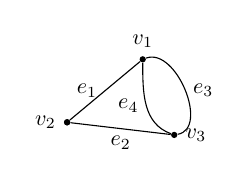
\begin{tikzpicture}[scale=0.8, every node/.style={transform shape}]
        \node[fill, circle, minimum size=1mm, inner sep=0] (O) at (0,0) {};
        \node[label=above:{$v_1$}, fill, circle, minimum size=1mm, inner sep=0] (v1) at (1.2,1) {};
        \node[label=left:{$v_2$}, fill, circle, minimum size=1mm, inner sep=0] (v2) at (0,0) {};
        \node[label=right:{$v_3$}, fill, circle, minimum size=1mm, inner sep=0] (v3) at (1.7,-0.2) {};
        \draw (v1) -- node[left] {$e_1$} (v2)
                   -- node[below] {$e_2$} (v3);
        \draw (v1) to[out=20, in=10] node[right] {$e_3$} (v3);
        \draw (v3) to[out=-200, in=-90] node[left] {$e_4$} (v1);
    \end{tikzpicture}
    \\* $e_1 = \{v_1, v_2\}$

    directed graph
    \\
    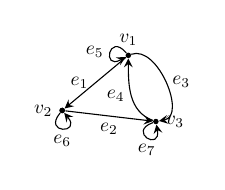
\begin{tikzpicture}[scale=0.7, every node/.style={transform shape}]
        \node[fill, circle, minimum size=1mm, inner sep=0] (O) at (0,0) {};
        \node[label=above:{$v_1$}, fill, circle, minimum size=1mm, inner sep=0] (v1) at (1.2,1) {};
        \node[label=left:{$v_2$}, fill, circle, minimum size=1mm, inner sep=0] (v2) at (0,0) {};
        \node[label=right:{$v_3$}, fill, circle, minimum size=1mm, inner sep=0] (v3) at (1.7,-0.2) {};
        \draw[->,>=stealth] (v1) -- node[left] {$e_1$} (v2);
        \draw[->,>=stealth] (v2) -- node[below] {$e_2$} (v3);
        \draw[->,>=stealth] (v1) to[out=20, in=10] node[right] {$e_3$} (v3);
        \draw[->,>=stealth] (v3) to[out=-200, in=-90] node[left] {$e_4$} (v1);
        \draw[->,>=stealth] (v1) to[in=-150,out=-230, loop] node[left] {$e_5$} (v1);
        \draw[->,>=stealth] (v2) to[in=-50,out=-130, loop] node[below] {$e_6$} (v2);
        \draw[->,>=stealth] (v3) to[in=-80,out=-160, loop] node[below] {$e_7$} (v3);
    \end{tikzpicture}
    \\* $e_1 = (v_1, v_2)$
\end{center}
\end{multicols}

\subsubsection{undirected graph}
\begin{itemize}
    \item denoted by $G = (V, E)$, comprising
    \begin{itemize}
        \item nonempty set of \textit{vertices/nodes}, $V = \{v_1, v_2, \dots, v_n\}$
        \item a set of \textit{edges}, $E = \{e_1, e_2, \cdots, e_k\}$
    \end{itemize}
    \item $e = \{v, w\}$ for an undirected edge $E$ incident on vertices $v$ and $w$
\end{itemize}

\subsubsection{directed graph}
\begin{itemize}
    \item denoted by $G = (V, E)$, comprising
    \begin{itemize}
        \item nonempty set $V$ of \textit{vertices}
        \item a set $E$ of \textit{directed edges} (ordered pair of vertices)
    \end{itemize}
    \item $e = (v, w)$ : an directed edge $E$ from vertex $v$ to vertex $w$
\end{itemize}

\subsubsection{simple graph}
\begin{itemize}
    \item \textbf{undirected graph} with no loops or parallel edges
\end{itemize}

\subsubsection{complete graph}
\begin{itemize}
    \item a complete graph on $n$ vertices, $n>0$, denoted $K_n$, is a simple graph with $n$ vertices and exactly one edge connecting each pair of distinct vertices
\end{itemize}

\subsubsection{subgraph of a graph}
$H$ is a subgraph of $G \Iff$ 
\begin{itemize}
    \item every vertex in $H$ is also a vertex in $G$
    \item every edge in $H$ is also an edge in $G$
    \item every edge in $H$ has the same endpoints as it has in $G$
\end{itemize}

\subsection{paths and walks}
Let $G$ be a graph; let $v$ and $w$ be vertices of $G$.
\begin{itemize}
    \item \textbf{path} (from $v$ to $w$): links two vertices in a graph via a sequence of edges, with no repeated vertices
    \\($\{x_0, x_1, \dots , x_l\}, \{x_0x_1, x_1x_2, \dots , x_{l-1}x_l\}$) where $v = x_0$ and $w = x_l$
    \begin{itemize}
        \item \textbf{length} of walk: the number of edges, $l$
        \item each vertex in a path is in at most 2 edges in the path
    \end{itemize}
    \item If there is a path P between $u$ and $v$, and path G between $v$ and $w$. Then there is a path between $u$ and $w$
\end{itemize}

\subsection{cycles}
\begin{itemize}
    \item \textbf{circuit/cycle}: an undirected graph $G(V, E)$ where 
    \begin{itemize}
        \item $V = \{x_1, x_2, \dots, x_l\}$
        \item $E = \scriptstyle \{\{x_1, x_2\}, \{x_2, x_3\}, \dots, \{x_{l-1}, x_l\}, \{x_l, x_1\}\}$
        \item $n \in \mathbb{Z}_{\geq 3}$
    \end{itemize}
    \item \textbf{simple circuit/cycle}: does not have any other repeated vertex except the first and last
    \item An undirected graph is \textbf{cyclic} if it contains a loop/cycle
    \item An undirected graph is with no loop is cyclic iff it has two vertices between which there are two distinct paths
\end{itemize}


\subsection{connectedness} 
\begin{itemize}
    \item vertices $v$ and $w$ are connected $\Iff \exists$ a path from $v$ to $w$
    \item graph $G$ is connected $\Iff \forall$ vertices $v, w \in V, \exists$ a path from $v$ to $w$ 
\end{itemize}
\subsubsection{connected component}
\begin{itemize}
    \item a connected subgraph of the largest possible size
    \item graph $H$ is a connected component of graph $G \Iff$ 
    \begin{enumerate}
        \item $H$ is a subgraph of $G$
        \item $H$ is connected
        \item no connected subgraph of $G$ has $H$ as a subgraph and contains vertices or edges that are not in $H$
    \end{enumerate}
    \item Let G be an undirected graph, then every vertex $v$ in $G$ is in some connected component of $G$
    \item Let $u,v$ be vertices in an undirected graph $G$. Then there is a path between $u$ and $v$ in G $\iff$ there is a connected component $G$ that has both $u$ and $v$ in it
\end{itemize}

\subsubsection{counting walks of length N}
\begin{center}
    number of walks of length $n$ from $v_i$ to $v_j$ 
    \\* $=$ the $ij$-th entry of $A^n$
\end{center}

\subsection{isomorphism}
\begin{itemize}
    \item graph isomorphism ($\cong$) is an equivalence relation.
\end{itemize}
\begin{center}
Let $G = (V_G, E_G)$ and $G' = (V_{G'}, E_{G'})$ be two graphs.
    \\* $G \cong G' \Iff$ there exist bijections $g: V_G \to V_G'$ and $h: E_G \to E_G'$ that preserve
        the edge-edgepoint functions of $G$ and $G'$ in the sense that $\forall v \in V_G$ and $e \in E_G$,
    \\* $v$ is an endpoint of $e \Iff g(v)$ is an endpoint of $h(e)$.
\end{center}

\section{12. TREES}
\begin{itemize}
    \item \textbf{tree} is a \textbf{connected acyclic undirected} graph
    \begin{itemize}
        \item If $G$ is a connected graph with $n$ vertices and $n-1$ edges, then $G$ is a tree.
    \end{itemize}
    \item \textbf{terminal vertex / leaf}: vertex with no child
    \item \textbf{internal vertex / parent}: vertex that is not terminal
\end{itemize}

\begin{center}
    \begin{multicols}{3}
        graph
        \\*
        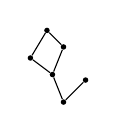
\begin{tikzpicture}[scale=0.7, every node/.style={transform shape}]
            \node[fill, circle, minimum size=1mm, inner sep=0] (v1) at (0,1) {};
            \node[fill, circle, minimum size=1mm, inner sep=0] (v2) at (0.3,1.5) {};
            \node[fill, circle, minimum size=1mm, inner sep=0] (v3) at (0.4,0.7) {};
            \node[fill, circle, minimum size=1mm, inner sep=0] (v4) at (0.6,1.2) {};
            \node[fill, circle, minimum size=1mm, inner sep=0] (v5) at (0.6,0.2) {};
            \node[fill, circle, minimum size=1mm, inner sep=0] (v6) at (1,0.6) {};
            \draw (v3) -- (v1) -- (v2) -- (v4) -- (v3) -- (v5) -- (v6);
        \end{tikzpicture}
        
        tree
        \\*
        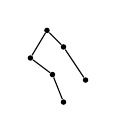
\begin{tikzpicture}[scale=0.7, every node/.style={transform shape}]
            \node[fill, circle, minimum size=1mm, inner sep=0] (v1) at (0,1) {};
            \node[fill, circle, minimum size=1mm, inner sep=0] (v2) at (0.3,1.5) {};
            \node[fill, circle, minimum size=1mm, inner sep=0] (v3) at (0.4,0.7) {};
            \node[fill, circle, minimum size=1mm, inner sep=0] (v4) at (0.6,1.2) {};
            \node[fill, circle, minimum size=1mm, inner sep=0] (v5) at (0.6,0.2) {};
            \node[fill, circle, minimum size=1mm, inner sep=0] (v6) at (1,0.6) {};
            \draw (v5) -- (v3) -- (v1) -- (v2) -- (v4) -- (v6);
        \end{tikzpicture}
        
        forest
        \\*
        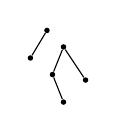
\begin{tikzpicture}[scale=0.7, every node/.style={transform shape}]
            \node[fill, circle, minimum size=1mm, inner sep=0] (v1) at (0,1) {};
            \node[fill, circle, minimum size=1mm, inner sep=0] (v2) at (0.3,1.5) {};
            \node[fill, circle, minimum size=1mm, inner sep=0] (v3) at (0.4,0.7) {};
            \node[fill, circle, minimum size=1mm, inner sep=0] (v4) at (0.6,1.2) {};
            \node[fill, circle, minimum size=1mm, inner sep=0] (v5) at (0.6,0.2) {};
            \node[fill, circle, minimum size=1mm, inner sep=0] (v6) at (1,0.6) {};
            \draw (v1) -- (v2);
            \draw (v5) -- (v3) -- (v4) -- (v6);
        \end{tikzpicture}
    \end{multicols}
\end{center}

\subsection{rooted trees}
\begin{itemize}
    \item \textbf{rooted tree}: a tree in which there a distinguished vertex called the root.
    \item \textbf{height} (of a rooted tree): length of a longest path between root and some vertex
\end{itemize}

\subsubsection{binary tree}
\begin{itemize}
    \item \textbf{binary tree}: a rooted tree in which every parent has at most 2 children
    \begin{itemize}
        \item at most one left child and at most one right child
    \end{itemize}
    \item \textbf{full binary tree}: a binary tree in which every parent has exactly 2 children
    \item (left/right) \textbf{subtree}: Given any parent $v$ in a binary tree $T$, 
        the binary tree whose root is the (left/right) child of $v$, whose vertices consist of the left child of $v$ and all its descendants, 
        and whose edges consist of all those edges of $T$ that connect the vertices of the left subtree.
\end{itemize}
\begin{center}
    \textbf{T10.6.1}: Full Binary Tree Theorem
    \\* If $T$ is a full binary tree with $k$ internal vertices, then $T$ has a total of $2k + 1$ vertices and has $k+1$ terminal vertices.
\end{center}

\subsubsection{binary tree traversal}
\noindent
\begin{minipage}[c]{0.3\linewidth}
    \begin{center}
        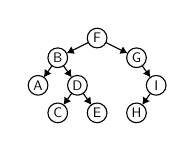
\begin{tikzpicture}[scale=0.5, every node/.style={transform shape}]
            \node[draw, circle, minimum size=5mm, inner sep=0pt, outer sep=0pt] (F) at (0,0) {F};
            \node[draw, circle, minimum size=5mm, inner sep=0pt, outer sep=0pt] (B) at (-1,-0.5) {B};
            \node[draw, circle, minimum size=5mm, inner sep=0pt, outer sep=0pt] (G) at (1,-0.5) {G};
            \node[draw, circle, minimum size=5mm, inner sep=0pt, outer sep=0pt] (A) at (-1.5,-1.2) {A};
            \node[draw, circle, minimum size=5mm, inner sep=0pt, outer sep=0pt] (D) at (-0.5,-1.2) {D};
            \node[draw, circle, minimum size=5mm, inner sep=0pt, outer sep=0pt] (I) at (1.5,-1.2) {I};
            \node[draw, circle, minimum size=5mm, inner sep=0pt, outer sep=0pt] (C) at (-1,-1.9) {C};
            \node[draw, circle, minimum size=5mm, inner sep=0pt, outer sep=0pt] (E) at (0,-1.9) {E};
            \node[draw, circle, minimum size=5mm, inner sep=0pt, outer sep=0pt] (H) at (1,-1.9) {H};
            \draw[-{Latex[angle=60:3pt]}] (F) -- (B);
            \draw[-{Latex[angle=60:3pt]}] (F) -- (G);
            \draw[-{Latex[angle=60:3pt]}] (B) -- (A);
            \draw[-{Latex[angle=60:3pt]}] (B) -- (D);
            \draw[-{Latex[angle=60:3pt]}] (D) -- (C);
            \draw[-{Latex[angle=60:3pt]}] (D) -- (E);
            \draw[-{Latex[angle=60:3pt]}] (G) -- (I);
            \draw[-{Latex[angle=60:3pt]}] (I) -- (H);
        \end{tikzpicture}
        \\ {\tiny\textit{F-B-G-A-D-I-C-E-H}}
    \end{center}
\end{minipage} % no space if you would like to put them side by side
\begin{minipage}[c]{0.65\linewidth}\color{black}
    \textbf{Breadth-First Search (BFS)}
    \begin{itemize}
        \item starts at the root 
        \item visits its adjacent vertices
        \item visits the next level
    \end{itemize}
\end{minipage}

\ 
\\ \textbf{Depth-First Search (DFS)}
\begin{itemize}
    \item \textbf{pre-order}
    \begin{itemize}
        % \item process the root (or current vertex)
        % \item traverse the left subtree recursively
        % \item traverse the right subtree recursively
        \item current vertex $\then$ left subtree $\then$ right subtree
    \end{itemize}
    \item \textbf{in-order}
    \begin{itemize}
        \item left subtree $\then$ current vertex $\then$ right subtree
    \end{itemize}
    \item \textbf{post-order}
    \begin{itemize}
        \item left subtree $\then$ right subtree $\then$ current vertex 
    \end{itemize}
\end{itemize}

\subsection{spanning trees}
\begin{itemize}
    \item \textbf{spanning tree} (for a graph $G$): a subgraph of $G$ that contains every vertex of $G$ and is a tree.
    \begin{itemize}
        \item $w(e)$ - weight of edge $e$
        \item $w(G)$ - total weight of $G$
    \end{itemize}
    \item \textbf{weighted graph}: each edge has an associated positive real number weight
    \begin{itemize}
        \item \textbf{total weight}: sum of the weights of all edges
    \end{itemize}
    \item \textbf{minimum spanning tree}: least possible total weight compared to all other spanning trees
\end{itemize}

\subsubsection{Kruskal's algorithm}
For a connected weighted graph $G$ with $n$ vertices:
\begin{enumerate}
    \item initialise $T$ to have all the vertices of $G$ and no edges.
    \item let $E$ be the set of all edges in $G$; let $m = 0$
    \item while $(m < n - 1)$
    \begin{enumerate}
        \item find and remove the edge $e$ in $E$ of least weight
        \item if adding $e$ to the edge set of $T$ does not produce a circuit:
        \begin{enumerate}
            \item add $e$ to the edge set of $T$
            \item set $m = m + 1$
        \end{enumerate}
    \end{enumerate}
\end{enumerate}

\subsubsection{Prim's algorithm}
For a connected weighted graph $G$ with $n$ vertices:
\begin{enumerate}
    \item pick any vertex $v$ of $G$ and let $T$ be the graph with this vertex only
    \item let $V$ be the set of all vertices of $G$ except $v$
    \item for ($i = 0$ to $n-1$)
    \begin{enumerate}
        \item find the edge $e$ in $G$ with the least weight of all the edges connected to $T$.
            let $w$ be the endpoint of $e$.
        \item add $e$ and $w$ to the edge and vertex sets of $T$
        \item delete $w$ from $v$
    \end{enumerate}
\end{enumerate}

\end{multicols}

\pagebreak

\begin{center}
    \begin{tabular}{>{\color{black}}r | c | c}
        \multicolumn{3}{>{\color{black}}c}{LOGICAL EQUIVALENCES} 
        \\ \hline 
        commutative laws 
            & $p \land q \equiv q \land p$
            & $p \lor q \equiv q \lor p$
        \\ associative laws
            & $(p \land q) \land r \equiv p \land (q \land r)$
            & $(p \lor q) \lor r \equiv p \lor (q \lor r)$
        \\ distributive laws
            & $p \land (q \lor r) \equiv (p \land q) \lor (p \land r)$
            & $p \lor (q \land r) \equiv (p \lor q) \land (p \lor r)$
        \\ identity laws
            & $p \land true \equiv p$
            & $p \lor false \equiv p$
        \\ idempotent laws
            & $p \land p \equiv p$
            & $p \lor p \equiv p$
        \\ annihilators laws
            & $p \lor true \equiv true$
            & $p \land false \equiv false$
        \\ negation laws
            & $p \lor \lnot p \equiv true$
            & $p \land \lnot p \equiv false$
        \\ double negation law
            & $\lnot (\lnot p) \equiv p$
            & —
        \\ absorption laws
            & $p \lor (p \land q) \equiv p$
            & $p \land (p \lor q) \equiv p$
        \\ De Morgan's Laws
            & $\lnot (p \lor q) \equiv \lnot p \land \lnot q $
            & $\lnot (p \land q) \equiv \lnot p \lor \lnot q$
        \\ Implication law
            & $p \rightarrow q \equiv \lnot p \lor q$
            & -
     \end{tabular}
     \quad
     \begin{tabular}{>{\color{black}}r | c | c}
        \multicolumn{3}{>{\color{black}}c}{SET IDENTITIES} 
        \\ \hline 
        commutative laws 
            & $A \cap B = B \cap A$
            & $A \cup B = B \cup A$
        \\ associative laws
            & $(A \cap B) \cap C = A \cap (B \cap C)$
            & $(A \cup B) \cup C = A \cup (B \cup C)$
        \\ distributive laws
            & $A \cap (B \cup C) = (A \cap B) \cup (A \cap C)$
            & $A \cup (B \cap C) = (A \cup B) \cap (A \cup C)$
        \\ identity laws
            & $A \cap U = A$
            & $A \cup \emptyset = A$
        \\ idempotent laws
            & $A \cap A = A$
            & $A \cup A = A$
        \\ annihilators laws
            & $A \cap \emptyset = \emptyset$
            & $A \cup U = U$
        \\ complement laws
            & $A \cap \overline{A} = \emptyset$
            & $A \cup \overline{A} = U$
        \\ double \bf{complement} law
            & $\overline{(\overline{A})} = A$
            & ---
        \\ absorption laws
            & $A \cup (A \cap B) = A$
            & $A \cap (A \cup B) = A$
        \\ De Morgan's Laws
            & $\overline{A \cup B} = \overline{A} \cap \overline{B}$
            & $\overline{A \cap B} = \overline{A} \cup \overline{B}$
        \\ Set difference
            & $A \backslash B \equiv A \cap \overline{B} $
            & -
     \end{tabular}
\end{center}
\begin{center}
    % \hrulefill \\
    \dotfill
\end{center}
\begin{multicols}{3}
    \section{proven:}
    \subsection{number theory}
    \begin{itemize}
        \item - the product of 2 consecutive odd numbers is always odd.
        \item - the difference between 2 consecutive squares is always odd
        \item P3.2.4 -  the square of any 2 even integers is even
        \item - there is no greatest integer
        \item - there are infinitely many prime numbers
        \item - for all positive integers $a$ and $b$, if $a \vert b$, then $a \leq b$.
        \item P3.2.8 - for all integers $n$, if $n^2$ is even then $n$ is even
        \item - all integers are rational numbers
        \item - the sum of any 2 rational numbers is rational
        \item - there exist irrational numbers $p$ and $q$ such that $p^q$ is rational
        \item - $\sqrt{2}$ is irrational.
        \item - the only divisors of $1$ are $1$ and $-1$.
    \end{itemize}
    \textbf{divisibility}
    \begin{itemize}
        \item L8.1.5 - Let $d, n \in \mathbb{Z}$ with $d \neq 0$. Then $d \mid n \Iff n/d \in \mathbb{Z}$ 
        \item L8.1.9 - Let $d, n \in \mathbb{Z}$. If $d \mid n$, then $-d \mid n$ and $d \mid -n$ and $-d \mid -n$ 
        \item L8.1.10 - Let $d, n \in \mathbb{Z}$. If $d \mid n$ and $d \neq 0$, then $\vert d \vert \leq \vert n \vert$ 
        \item L8.2.5 - \bf{Prime Divisor Lemma} (non-standard name):
        \begin{itemize}
            \item Let $n \in \mathbb{Z}_{\geq 2}$. Then $n$ has a prime divisor.
        \end{itemize}
        \item P8.2.6 - \bf{sizes of prime divisors}: 
        \begin{itemize}
            \item Let $n$ be a composite positive integer. Then $n$ has a prime divisor $p \leq \sqrt{n}$.
        \end{itemize}
    \end{itemize}

    \subsection{logic}
    \begin{itemize}
        \item negation of a universal statement: 
        \begin{itemize}
            \item $ \lnot \forall \: P(x) \iff \exists x \: \lnot P(x)$
        \end{itemize}
        \item negation of an existential statement: 
        \begin{itemize}
            \item $ \lnot \exists \: P(x) \iff \forall x \: \lnot P(x)$
        \end{itemize}
        \item negation for more predicates : 
        \begin{itemize}
            \item $ \lnot \forall x \exists y \: Q(x,y) \iff \exists x \forall y \: \lnot Q(x,y)$
        \end{itemize}
    \end{itemize}

    \subsection{sets}
    \begin{itemize}
        \item P4.2.7 - $\emptyset \subseteq $ all sets
        \item T4.1.18 - there exists a unique set with no element. It is denoted by $\emptyset$.
        \item E4.3.7 - for all $A, B$: $(A \cap B) \cup (A \backslash B) = A$
        \item E4.3.9(1) - ($A \cap B) \subseteq A$
        \item E4.3.9(2) - $A \subseteq (A \cup B$)
        \item E4.3.10 - $A \subseteq B \land B \subseteq C \rightarrow A \subseteq (B \cap C$)
        \item T4.6 - $A \subseteq B \iff A \cup B = B$
        \item T5.3.11(1) - let $A, B$ be disjoint finite sets. Then $\vert A \cup B \vert = \vert A \vert + \vert B \vert$
        \item T5.3.11(2) - let $A_1, A_2, \dots, A_n$ be pairwise disjoint finite sets. Then $\vert A_1 \cup A_2 \cup \dots \cup A_n \vert = \vert A_1 \vert + \vert A_2 \vert + \dots + \vert A_n \vert$
        \item T5.3.12 - \bf{Inclusion-Exclusion Principle}: 
        \begin{itemize}
            \item for all finite sets $A$ and $B$, $\vert A \cup B \vert = \vert A \vert + \vert B \vert - \vert A \cap B \vert$
        \end{itemize} 
    \end{itemize}

    \subsection{relations}
    \begin{itemize}
        \item E6.2.2 - The equality relation $R$ on a set $A$ has equivalence classes of the form $[x] = \{y \in A : x = y \} = \{x\}$ where $x \in A$
        \item L6.3.11 - Let $R$ be an equivalence relation on a set $A$. Then $A / R$ is a partition of A.
        \item - If $\mathscr{C}$ is a partition of $A$, then there is an equivalence relation of $R$ on $A$ such that $A/R = \mathscr{C}$.
        \item L6.3.5 - Let $\lnot$ be an equivalence relation a set $A$.
        \begin{itemize}
            \item $x \in [x] $ for all $ x \in A$
            \item any equivalence class is non empty
        \end{itemize}
        \item L6.3.6 - $\forall x,y \in A \: $ if $(x] \cap [y] \neq \emptyset$ , then $[x] = [y]$
        \item - Consider a partial order $\preccurlyeq$ on set $A$. 
        \begin{itemize}
            \item A smallest element is minimal.
            \item There is at most one smallest element.
        \end{itemize}
        \item T6.4 - $x \lnot y \iff [x] = [y]$ , where $\lnot$ is an equivalence relation
        \item P7.4.3 - if $f$ is a bijection $A \then B$ , then $f^{-1}$ is a bijection $B \then A$
    \end{itemize}

    \subsection{functions}
    \begin{itemize}
        \item P7.4.13 - $f \circ \text{id}_\text{A} = f$ and $\text{id}_\text{A} \circ f = f$
        \item P7.4.3 - if $f$ is a bijection $A \then B$ , then $f^{-1}$ is a bijection $B \then A$ 
        \item T7.6 - if $f$ is surjective, and $g \circ f =  \text{id}_\text{A}$, then $g$ is injective
        \item E7.9 - Let $f : A \then B$. if $f^{-1}$ is a function $B \then A$ , then $f^{-1}$ is bijective
        \item range($f$) $\in$ codomain
        \item if $f$ is surjective: range($f$) $\in$ codomain $\in$ range($f$)
    \end{itemize}
    
    \subsection{graphs and trees}
    \begin{itemize}
        \item - Let $G$ be a graph.
        \begin{itemize}
            \item - If $G$ is connected, then any two distinct vertices of $G$ can be connected by a path
            \item T12.1.4 - A connected undirected graph $G$ is a tree $\iff$ removing any edge disconnects $G$
            \item - If $G$ is connected and $G$ contains a circuit, then an edge of the circuit can be removed without disconnecting $G$.
        \end{itemize}
        \item T12.1.4 - If $G$ is any connected graph, $C$ is any circuit in $G$, and one of the edges of $C$ is removed from $G$, then the graph that remains is still connected.
        \item T12.1.6 - Let $G$ be finite tree with $>$ 1 vertex, $|E(G)| = |V(G)| - 1$
        \item T12.1.8 - Let $G$ be a connected cyclic finite undirected graph, then $|E(G)| \geq |V(G)|$
        \item P12.2.3 - Let $T$ be a finite rooted tree of heigh $h$ in which every vertex has at most 2 children, then $T$ has at most $2^h$ terminal vertices.
        \item P12.2.5 - Let $T$ be a finite rooted tree in which every vertex has exactly 2 children. If $T$ has exactly $t$ terminal vertices, then $T$ has exactly $t-1$ internal vertices and thus exactly $2t-1$ vertices in total
        \item Tut12.9 - Let $T$ be a finite tree with at least 2 vertices. $T$ has at least 2 vertices that are each in exactly one edge.
        \item - If $T$ is a full binary tree with $k$ internal vertices, then $T$ has a total of $2k + 1$ vertices and has $k+1$ terminal vertices.
    \end{itemize}

\begin{center}
    \fbox{%
        \parbox{0.3\linewidth}{\textcolor{black}{%
            {\large abbreviations}
            \begin{itemize}
                \item L - lemma
                \item E - example
                \item P - proposition
                \item T - theorem
            \end{itemize}
        }}%
    }
\end{center}
\end{multicols}

\end{document}